\part{微分几何}\label{Part:Differential_Geometry}
	\begin{margintable}\vspace{1.4in}\footnotesize
		\begin{tabularx}{\marginparwidth}{|X}
			
			%Section~\ref{sec:structure}. 张量场与微分形式场\\
			Section~\ref{sec:Riemannian_Manifold}. Riemannian流形\\
			
			%Section~\ref{sec:LieAlgebra}. 联络与曲率\\
		\end{tabularx}
	\end{margintable}
	我并不打算像通常的微分几何教程那样循规蹈矩,而是用一种我认为通俗易懂的描述构造non-Euclidean几何框架.当然,这样做会损失一些数学上的严谨性,但我认为这对于物理工作者而言无伤大雅.
	\section{坐标系}
		我们首先回顾一下线性空间的公理化定义.
		\begin{definition}
			域$F$上的线性空间$V$是这样一个集合,对任意$\alpha,\beta,\gamma\in V;a,b\in F$满足
			\begin{enumerate}
				矢量加法映射$V\times V\rightarrow V$:
				\item (交换律)$\alpha+\beta=\beta+\alpha$;
				\item (结合律)$(\alpha+\beta)+\gamma=\alpha+(\beta+\gamma)$;
				\item (零元)存在唯一的$0\in V$,使得$0+\alpha=\alpha$;
				\item (逆元)对任意$\alpha\in V$,存在唯一的$\beta\in V$,使得$\alpha+\beta=0$.
				
				矢量数乘映射$F\times V\rightarrow V$:
				\item (酉性)对$1\in F$,有$1\alpha=\alpha$;
				\item (结合律)$a(b\alpha)=(ab)\alpha$;
				\item (分配律1)$(a+b)\alpha=a\alpha+b\alpha$;
				\item (分配律2)$a(\alpha+\beta)=a\alpha+a\beta$.
			\end{enumerate}
		\end{definition}
		在第一次学习这个定义的时候,你可能会问:“这有什么意义?交换律,结合律,分配律,这些东西不是小学就学了么?”这就是公理化的奇妙之处.我们总是能从这样通俗易懂的基础逻辑出发,演绎出宏伟的结构.数学是这样,后面我们会看到理论物理(而不是材料物理)也是这样.
		
		一个最平凡的例子就是$n$维Euclidean空间$\mathbb{R}^n$.我们将$\mathbb{R}^n$中的元素称为\textbf{点},记为一个有序数组$(x^1,\cdots,x^n)$,或简记为$(x^\mu),\mu=1,\cdots,n$,其中$x^\mu$是$n$个称为\textbf{坐标}的实参数.容易证明$\mathbb{R}^n$完全满足线性空间的定义.
		
		事实上我们还可以引入不同的参数来表示空间中的同一点.例如,我们找来一组带撇的参数$x'^\mu$,然后将原来的$(x^1,\cdots,x^n)$转换为$(x'^1,\cdots,x'^n)$,这个过程称为\textbf{坐标变换},我们可以用一个映射$\varphi$表示之\footnote{通常会对这一映射加上某些光滑、可逆的限制.}:
		\begin{equation}\label{eq:coordinate transformation}
			\varphi:\mathbb{R}^n\rightarrow \mathbb{R}^n,(x^1,\cdots,x^n)\mapsto (x'^1,\cdots,x'^n).
		\end{equation}
		我们注意到(\ref{eq:coordinate transformation})这个映射相当于“输入$(x^1,\cdots,x^n)$,得到$x'^1$;$\cdots$;输入$(x^1,\cdots,x^n)$,得到$x'^n$”,而这等价于$n$个$n$元函数:
		\begin{equation}
			\begin{split}
				\varphi^1&:\mathbb{R}^n\rightarrow \mathbb{R},(x^1,\cdots,x^n)\mapsto x'^1;\\
				&\cdots\\
				\varphi^n&:\mathbb{R}^n\rightarrow \mathbb{R},(x^1,\cdots,x^n)\mapsto x'^n.
			\end{split}
		\end{equation}
		这就是通常意义下的坐标变换函数组.
		
		我们说,每一组参数组$(x^\mu)$都对应了一种参数坐标系.假设某组参数确定了一个$\mathbb{R}^n$中的点,当我们固定$n-1$个参数$x^{\mu_1},\cdots,x^{\mu_{i-1}},x^{\mu_{i+1}},\cdots,x^{\mu_n}$,只让一个参数$x^i$变化时,这个点就走出了一条轨迹.我们将这条轨迹称为坐标$x^i$的\textbf{坐标线}.对于$\mathbb{R}^3$,我们可以将坐标系画下来.
		\subsection{直角坐标系}
		\begin{marginfigure}
			\centering
			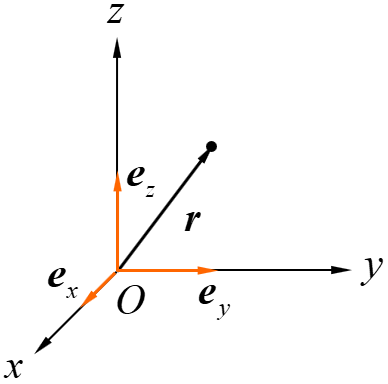
\includegraphics[width=1\textwidth]{figures/rectangular_coordinates.png}
			\caption{直角坐标系}\label{fig:rectangular_coordinates}
		\end{marginfigure}
		最典型的例子就是正交直角坐标系,或者说是Cartesian坐标系,如图\ref{fig:rectangular_coordinates}所示.在这种坐标系中,坐标线是直线,且彼此正交.通常,我们用$(x,y,z)$来表述直角坐标系中的点.
		\subsection{柱坐标系}
		\begin{marginfigure}
			\centering
			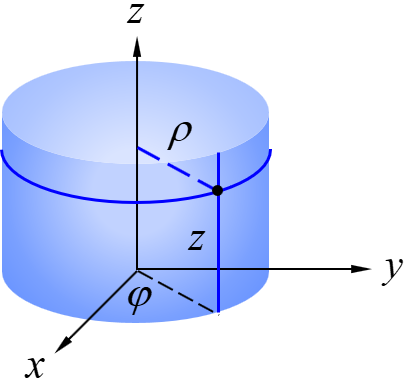
\includegraphics[width=1\textwidth]{figures/cylindrical_coordinates.png}
			\caption{柱坐标系}\label{fig:cylindrical_coordinates}
		\end{marginfigure}
		柱坐标系如图\ref{fig:cylindrical_coordinates}所示.通常,我们用$(r,\theta,z)$来表述柱坐标系中的点,其中线参数$r\in[0,+\infty)$,$z\in \mathbb{R}$,角参数$\theta\in[0,2\pi)$,这些参数构成的坐标线彼此正交.将一个由柱坐标参数描述的点变换到由直角坐标参数描述的点总是容易的,我们有它的坐标变换映射
		\begin{equation}\label{eq:rthetaz to xyz 1}
			(r,\theta,z)\mapsto(x,y,z),
		\end{equation}
		用坐标变换函数组表示就是
		\begin{equation}\label{eq:rthetaz to xyz 2}
			\begin{split}
				x(r,\theta,z)&=rCos\theta;\\
				y(r,\theta,z)&=rSin\theta;\\
				z(r,\theta,z)&=z.
			\end{split}
		\end{equation}
		我们注意到\ref{eq:rthetaz to xyz 2}是光滑的,这意味着它还是可逆的.于是我们可以得到\ref{eq:rthetaz to xyz 1}的逆映射
		\begin{equation}\label{eq:xyz to rthetaz 1}
			(x,y,z)\mapsto(r,\theta,z),
		\end{equation}
		用坐标变换函数组表示就是
		\begin{equation}\label{eq:xyz to rthetaz 2}
			\begin{split}
				r(x,y,z)&=\sqrt{x^2+y^2};\\
				\theta(x,y,z)&=Arccos\left(\frac{x}{\sqrt{x^2+y^2}}\right);\\
				z(x,y,z)&=z.
			\end{split}
		\end{equation}
		
		\subsection{球坐标系}
		
		\begin{marginfigure}
			\centering
			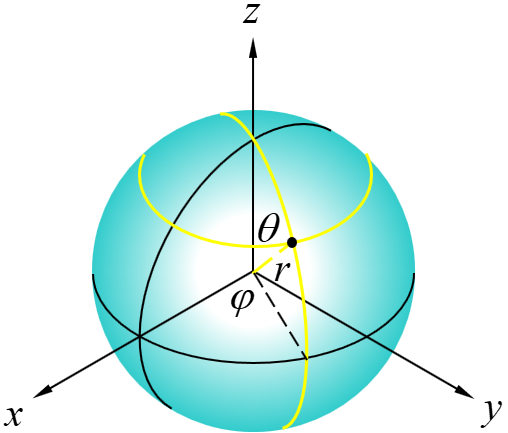
\includegraphics[width=1\textwidth]{figures/spherical_coordinates.png}
			\caption{球坐标系}\label{fig:spherical_coordinates}
		\end{marginfigure}
		球坐标系是除了直角坐标系以外最常用的坐标系,如图\ref{fig:spherical_coordinates}所示.我们用$(r,\theta,\varphi)$来描述球坐标系中的点,其中线参数$r\in[0,+\infty)$,角参数$\theta\in[0,\pi)$,$\varphi\in[0,2\pi)$,两个角参数通常隐含着系统的球对称性以及各向同性.与柱坐标系相同,球坐标系到直角坐标系也有坐标变换映射
		\begin{equation}\label{eq:rthetaphi to xyz 1}
			(r,\theta,\varphi)\mapsto(x,y,z),
		\end{equation}
		用坐标变换函数组表示就是
		\begin{equation}\label{eq:rthetaphi to xyz 2}
			\begin{split}
				x(r,\theta,\varphi)&=rSin\theta Cos\varphi;\\
				y(r,\theta,\varphi)&=rSin\theta Sin\varphi;\\
				z(r,\theta,\varphi)&=rCos\theta.
			\end{split}
		\end{equation}
		同样的有直角坐标系到球坐标系的逆变换
		\begin{equation}\label{eq:xyz to rthetaphi 1}
			(r,\theta,\varphi)\mapsto(x,y,z),
		\end{equation}
		用坐标变换函数组表示就是
		\begin{equation}\label{eq:xyz to rthetaphi 2}
			\begin{split}
				r(x,y,z)&=\sqrt{x^2+y^2+z^2};\\
				\theta(x,y,z)&=Arccos\left(\frac{z}{\sqrt{x^2+y^2+z^2}}\right);\\
				\varphi(x,y,z)&=Arctan(\frac{y}{x}).
			\end{split}
		\end{equation}

		$n$维的超球坐标系由$1$个线参数$y^1\in[0,+\infty)$和$n-1$个角参数$y^2,\dots,y^{n-2}\in[0,\pi)$,$y^{n-1}\in[0,2\pi)$构成.超球坐标系到直角坐标系的坐标变换由如下映射给出
		\begin{equation}
			\phi:R^n\rightarrow R^n;(y^1,\dots,y^n)\mapsto(x^1,\dots,x^n),
		\end{equation}
		用坐标变换函数组表示就是
		\begin{equation}\label{eq:xyz to rthetaphi 2}
			\begin{split}
				&x^1=y^1Cosy^2;\\
				&x^2=y^1Siny^2Cosy^3;\\
				&x^3=y^1Siny^2Siny^3Cosy^4;\\
				&\dots\\
				&x^{n-1}=y^1Siny^2\dots Siny^{n-2}Cosy^{n-1};\\
				&x^{n-1}=y^1Siny^2\dots Siny^{n-2}Siny^{n-1}.
			\end{split}
		\end{equation}




		\section{切空间与余切空间}
		现在,我们正式引入切空间.


		



	\section{张量场与微分形式场}


	\section{Riemannian流形}\label{sec:Riemannian_Manifold}
		一个流形指的是这样一个结构,其在局部上是平直的,但整体不必是平直的,为了描述这一属性,我们引入度规张量.


	\section{联络与曲率}
		对于任意标量场$\phi\in \varGamma(T_{(0,0)}M)$,其外微分$d\phi$仍是是一个张量场
		\begin{equation}
				 d\phi=\frac{\partial\phi}{\partial x^\mu}dx^\mu=\frac{\partial\phi}{\partial {x}^\mu}\frac{\partial{x}^\mu}{\partial {x'}^\nu}d{x'}^\nu=\frac{\partial{\phi'}}{\partial {x'}^\nu}d{x'}^\nu\in \varGamma(T_{(0,1)}M),
		\end{equation}
		这意味着$d\phi$仍是张量丛截面的元素,用学物理家的话来说也就是$d\phi$仍然满足张量的变换规律.
		
		一个自然的问题是,对于切矢量场或余切矢量场,其外微分是否仍然是张量丛截面的元素?但问题就出在这,外微分算子是一个定义在外形式丛截面上的线性算子,切矢量场不是外形式丛截面中的元素,因此我们无法对一个切矢量场求外微分;余切矢量场作为1微分形式场,虽然它是外形式丛截面的元素,但它只是一种全反对称的张量场,我们无法对一个一般的非全反对称张量场求外微分.这些困难意味着我们需要推广外微分算子,寻找一个定义在一般张量丛截面$\varGamma(T_{(p,q)}M)$上的线性微分算子,让我们能对那些不在外形式丛截面中的张量场进行“微分”运算.这样构造的线性微分算子就是\textbf{仿射联络}.
		\begin{remark}
		余切矢量场$\omega\in \varGamma(T_{(0,1)}M)$在局部坐标系改变时满足
		\begin{equation}\label{eq:domega1}
				\omega=\omega_\mu dx^\mu=\omega_\mu\frac{\partial{x}^\mu}{\partial {x'}^\nu}d{x'}^\nu=\omega'_\nu d{x'}^\nu,
		\end{equation}
		我们对(\ref{eq:domega1})求全微分得到
		\begin{eqnarray}\label{eq:domega2}
			d\omega &=&d\omega'_\nu{\wedge}d{x'}^\nu\notag\\
			&=&d\left(\omega_\mu\frac{\partial{x}^\mu}{{\partial}{x'}^\nu}\right)\wedge d{x'}^\nu\notag\\
			&=&\frac{\partial{x}^\mu}{{\partial}{x'}^\nu}d\omega_\mu{\wedge}d{x'}^\nu+\omega_{\mu}d\left(\frac{\partial{x}^\mu}{\partial {x'}^\nu}\right){\wedge}d{x'}^\nu\notag\\
			&=&\left(\frac{\partial{\omega}_\mu}{{\partial}{x}^\sigma}\frac{\partial{x}^\sigma}{\partial {x'}^\rho}\frac{\partial{x}^\mu}{{\partial}{x'}^\nu}+{\omega}_\mu\frac{\partial^2{x}^\mu}{\partial {x'}^\rho{\partial}{x'}^\nu}\right)d{x'}^\rho{\wedge}d{x'}^\nu\\
			&=&\frac{\partial\omega'_\nu}{{\partial}{x'}^\rho}d{x'}^\rho{\wedge}d{x'}^\nu\notag,
		\end{eqnarray}
		注意到\ref{eq:domega2}中产生了一个二阶偏微分项,与张量的变换规律对比可知,这一项破坏了张量的变换规律.但外微分形式场的全反对称特性可以消除掉这一项带来的影响,即
		\begin{eqnarray}
			\frac{\partial\omega'_\nu}{{\partial}{x'}^\rho}d{x'}^\rho{\wedge}d{x'}^\nu&=&2\partial'_{[\rho}\omega'_{\nu]}{dx'}^{\rho}\otimes{dx'}^\nu\notag\\
				&=&2\left(\partial_{[\sigma}\omega_{\mu]}\frac{\partial{x}^\sigma}{\partial {x'}^\rho}\frac{\partial{x}^\mu}{{\partial}{x'}^\nu}+{\omega}_\mu\frac{\partial^2{x}^\mu}{\partial {x'}^{[\rho}{\partial}{x'}^{\nu]}}\right){dx'}^{\rho}\otimes{dx'}^\nu\notag\\
			&=&2\partial_{[\sigma}\omega_{\mu]}\frac{\partial{x}^\sigma}{\partial {x'}^\rho}\frac{\partial{x}^\mu}{{\partial}{x'}^\nu}{dx'}^{\rho}\otimes{dx'}^\nu,
		\end{eqnarray}
		所以$d\omega$实际上仍是张量场.但微分形式场说到底只是一种特殊的全反对称张量场,对于一般的张量场,我们无法通过张量场自身的对称性消除上述二阶偏微分项.
		\end{remark}

		现代微分几何中的联络指的是一般矢量丛上的联络.这一节我们先讨论切丛$T_{(1,0)}(M)$上的联络(称为\textbf{仿射联络}),然后逐步构造出张量丛$T_{(p,q)}(M)$上的联络.下面,我们直接给出仿射联络的定义.
		\begin{definition}
			仿射联络是一个映射
			\begin{equation*}
				D:\varGamma(T_{(1,0)}M)\rightarrow \varGamma(T_{(1,1)}M),
			\end{equation*}
			它满足下列条件:
			\begin{enumerate}
				\item 对任意的$A,B\in \varGamma(T_{(1,0)}M)$有 D(A+B)=D(A)+D(B);						
				\item 对任意的$A\in \varGamma(T_{(1,0)}M),\alpha\in \varGamma(T_{(0,0)}M)$有$D(\alpha A)=d\alpha\otimes A+\alpha D(A)$.
			\end{enumerate}
		\end{definition}
		局部上,联络由一组1微分形式给出.我们先来看自然标架场$\{\partial_\mu\}$的联络,命
		\begin{equation}
		D(\partial_\mu)=\omega^\rho_\mu \otimes\partial_\rho={\varGamma^\rho}_{\mu\nu}dx^\nu\otimes \partial_\rho,
		\end{equation} 
		其中$\omega^\rho_\mu={\varGamma^\rho}_{\mu\nu}dx^\nu$,${\varGamma^\rho}_{\mu\nu}$称为\textbf{联络系数},它是局部坐标系中的光滑函数.将$\omega^\rho_\mu$作为矩阵$\omega$第$\rho$行第$\mu$列的元素,这样构造的矩阵$\omega$称为\textbf{联络方阵}.可见,任意两个联络间的差异完全体现在联络方阵上.现在,我们来看联络的变换规律.在标架变换下,由联络的定义立即得到
		\begin{eqnarray}
			D(\partial'_\nu)&=&D\left(\frac{\partial{x^\mu}}{\partial{x'}^\nu}{\partial}_\mu\right)\notag\\
			&=&d\left(\frac{\partial{x^\mu}}{\partial{x'}^\nu}\right)\otimes{\partial}_\mu+\frac{\partial{x^\mu}}{\partial{x'}^\nu}D\left({\partial}_\mu\right)\notag\\
			&=&\left[d\left(\frac{\partial{x^\rho}}{\partial{x'}^\nu}\right)+\frac{\partial{x^\mu}}{\partial{x'}^\nu}\omega^\rho_\mu\right]\otimes{\partial}_\rho\notag\\
			&=&\left[d\left(\frac{\partial{x^\rho}}{\partial{x'}^\nu}\right)\frac{\partial{{x'}^\sigma}}{\partial{x^\rho}}+\frac{\partial{x^\mu}}{\partial{x'}^\nu}\omega^\rho_\mu\frac{\partial{{x'}^\sigma}}{\partial{x^\rho}}\right]\otimes\partial'_\sigma\notag\\
			&=&{\omega'}^\sigma_\nu\otimes\partial'_\sigma,
		\end{eqnarray}
		其中
		\begin{equation}\label{eq:connection}
		{\omega'}^\sigma_\nu=d\left(\frac{\partial{x^\rho}}{\partial{x'}^\nu}\right)\frac{\partial{{x'}^\sigma}}{\partial{x^\rho}}+\frac{\partial{x^\mu}}{\partial{x'}^\nu}\omega^\rho_\mu\frac{\partial{{x'}^\sigma}}{\partial{x^\rho}},
		\end{equation}
		这就是联络方阵在局部标架场改变时的变换公式.我们还可以进一步展开(\ref{eq:connection}),得到
		\begin{equation}
		{{\varGamma'}^\sigma}_{\nu\lambda}=\frac{\partial^2{x^\rho}}{\partial{x'}^\lambda\partial{x'}^\nu}\frac{\partial{{x'}^\sigma}}{\partial{x^\rho}}+{\varGamma^\rho}_{\mu\alpha}\frac{\partial{x^\mu}}{\partial{x'}^\nu}\frac{\partial{x}^\alpha}{\partial{x'}^\lambda}\frac{\partial{{x'}^\sigma}}{\partial{x^\rho}},
		\end{equation}
		这正是通常意义下的联络变换公式.可见联络系数${\varGamma^\rho}_{\mu\nu}$并不是一个张量,但引入它能使$D(\partial_\mu)$遵循张量的变换规律.
		
		稍作思考可以发现,若使用全反对称化的技巧,我们也能利用联络系数构造出一个张量.我们将在稍后给出具体讨论.

		切丛截面的联络在余切丛截面上诱导出一个联络(仍记为$D$),易看出它是从$\varGamma(T_{(0,1)}M)$到\\$\varGamma(T_{(0,2)}M)$的映射.
		现在现在我们来考察$\{\partial_\mu\}$的对偶标架$\{dx^\mu\}$的联络.$D(dx^\mu)$由下式确定
		$$d\left(\partial_\mu,dx^\nu\right)=\left(D(\partial_\mu),dx^\nu\right)+\left(\partial_\mu,D(dx^\nu)\right),$$
		我们设
		$$D(dx^\nu)={\omega^*}^\nu_\rho\otimes{dx}^\rho,$$
		于是
		$$\left(\partial_\mu,D(dx^\nu)\right)=\left(\partial_\mu,{\omega^*}^\nu_\rho\otimes{dx}^\rho\right)={\omega^*}^\nu_\rho\delta^\rho_\mu={\omega^*}^\nu_\mu.$$
		考虑到对偶标架满足
		$$\left(\partial_\mu,dx^\nu\right)=\delta^\nu_\mu,$$ 
		于是得到
		\begin{eqnarray}
			{\omega^*}^\nu_\mu&=&\left(\partial_\mu,D(dx^\nu)\right)=-\left(D(\partial_\mu),dx^\nu\right)\\
				&=&-\left(\omega^\rho_\mu\otimes\partial_\rho,dx^\nu\right)=-{\omega}^\rho_\mu\delta^\nu_\rho=-{\omega}^\nu_\mu,
		\end{eqnarray}
		即
		$D(dx^\nu)=-{\omega}^\nu_\rho\otimes{dx}^\rho$.
		至此,我们就能计算任意$A\in T_{(1,0)}(M)$与$B\in T_{(0,1)}(M)$的联络了.在局部坐标系下,我们有:			\begin{eqnarray}
			\begin{split}
				D(A)&=D(A^\mu\partial_\mu)\\
				&=dA^\mu\otimes\partial_\mu+A^{\mu}D(\partial_\mu)\\
				&=(\partial_{\rho}A^\mu+A^{\nu}{\varGamma^\mu}_{\nu\rho})dx^\rho{\otimes}\partial_\mu\\
				&=\nabla_{\rho}A^{\mu}dx^\rho{\otimes}\partial_\mu;
			\end{split}
		\end{eqnarray}
		\begin{eqnarray}
			\begin{split}
				D(B)&=D(B_{\mu}{dx}^\mu)\\
				&=dB_\mu\otimes{dx}^\mu+B_{\mu}D({dx}^\mu)\\
				&=(\partial_{\rho}B_\mu-B_\nu{\varGamma^\nu}_{\mu\rho})dx^\rho{\otimes}dx^\mu\\
				&=\nabla_{\rho}B_{\mu}dx^\rho{\otimes}dx^\mu,
			\end{split}
		\end{eqnarray}
		其中
		\begin{eqnarray}
			\nabla_{\rho}A^\mu&=&\partial_{\rho}A^\mu+A^{\nu}{\varGamma^\mu}_{\nu\rho};\\
				\nabla_{\rho}B_{\mu}&=&\partial_{\rho}B_\mu-B_\nu{\varGamma^\nu}_{\mu\rho}.
		\end{eqnarray}							
		这正是通常意义下的\textbf{协变导数}运算.由此可见,协变导数是一种依赖于局部坐标系的分量表述.用类似的方法,我们能得到$T_{(p,q)}(M)$上的诱导联络.
		\begin{definition}在一般张量丛$T_{(p,q)}M$上,由仿射联络诱导的联络是一个映射
			$$D:\varGamma(T_{(p,q)}M)\rightarrow\varGamma(T_{(p,q+1)}M),$$
			设任意$S\in \varGamma(T_{(p,q)}M)$,则$S$的联络在局部坐标系下满足
			\begin{equation}
				\begin{split}
					D(S)&=D({S^{\mu_1\dots\mu_p}}_{\nu_1\dots\nu_q}\partial_{\mu_1}\otimes\dots\otimes\partial_{\mu_p}\otimes{dx}^{\nu_1}\otimes\dots\otimes{dx}^{\nu_q})\\
				%&=d({S^{\mu_1\dots\mu_p}}_{\nu_1\dots\nu_q})\otimes\partial_{\mu_1}\otimes\dots\otimes\partial_{\mu_p}\otimes{dx}^{\nu_1}\otimes\dots\otimes{dx}^{\nu_q}\notag\\
				%&+{S^{\mu_1\dots\mu_p}}_{\nu_1\dots\nu_q}D(\partial_{\mu_1})\otimes\dots\otimes\partial_{\mu_p}\otimes{dx}^{\nu_1}\otimes\dots\otimes{dx}^{\nu_q}\notag\\
				%&+\dots+{S^{\mu_1\dots\mu_p}}_{\nu_1\dots\nu_q}\partial_{\mu_1}\otimes\dots\otimes D({\partial_{\mu_p}})\otimes{dx}^{\nu_1}\otimes\dots\otimes{dx}^{\nu_q}\notag\\
				%&+{S^{\mu_1\dots\mu_p}}_{\nu_1\dots\nu_q}\partial_{\mu_1}\otimes\dots\otimes{\partial_{\mu_p}}\otimes D({dx}^{\nu_1})\otimes\dots\otimes{dx}^{\nu_q}\notag\\
				%&+\dots+{S^{\mu_1\dots\mu_p}}_{\nu_1\dots\nu_q}\partial_{\mu_1}\otimes\dots\otimes{\partial_{\mu_p}}\otimes{dx}^{\nu_1}\otimes\dots\otimes D({dx}^{\nu_q})\notag\\
				%&=(\partial_\rho{S^{\mu_1\dots\mu_p}}_{\nu_1\dots\nu_q}+{S^{\sigma\dots\mu_p}}_{\nu_1\dots\nu_q}{\varGamma^{\mu_1}}_{\sigma\rho}\notag\\
				%&+\dots+{S^{\mu_1\dots\sigma}}_{\nu_1\dots\nu_q}{\varGamma^{\mu_p}}_{\sigma\rho}-{S^{\mu_1\dots\mu_p}}_{\sigma\dots\nu_q}{\varGamma^{\sigma}}_{\nu_1\rho}\notag\\
				%&-\dots-{S^{\mu_1\dots\mu_p}}_{\nu_1\dots\sigma}{\varGamma^{\sigma}}_{\nu_q\rho})dx^\rho\otimes\partial_{\mu_1}\otimes\dots\otimes\partial_{\mu_p}\otimes{dx}^{\nu_1}\otimes\dots\otimes{dx}^{\nu_q}\notag\\
				&=\nabla_{\rho}{S^{\mu_1\dots\mu_p}}_{\nu_1\dots\nu_q}dx^\rho\otimes\partial_{\mu_1}\otimes\dots\otimes\partial_{\mu_p}\otimes{dx}^{\nu_1}\otimes\dots\otimes{dx}^{\nu_q},
				\end{split}
			\end{equation}
			其中
			\begin{equation}
				\begin{split}
					\nabla_{\rho}{S^{\mu_1\dots\mu_p}}_{\nu_1\dots\nu_q}&=\partial_\rho{S^{\mu_1\dots\mu_p}}_{\nu_1\dots\nu_q}\\
					&+{S^{\sigma\dots\mu_p}}_{\nu_1\dots\nu_q}{\varGamma^{\mu_1}}_{\sigma\rho}+\dots+{S^{\mu_1\dots\sigma}}_{\nu_1\dots\nu_q}{\varGamma^{\mu_p}}_{\sigma\rho}\\
					&-{S^{\mu_1\dots\mu_p}}_{\sigma\dots\nu_q}{\varGamma^{\sigma}}_{\nu_1\rho}-\dots-{S^{\mu_1\dots\mu_p}}_{\nu_1\dots\sigma}{\varGamma^{\sigma}}_{\nu_q\rho}.
				\end{split}		
			\end{equation}
		\end{definition}


\newpage
	
	
	
		